\documentclass[10pt]{beamer}

%%%
% PREAMBLE FOR THIS DOC 
%%%
%https://tex.stackexchange.com/questions/68821/is-it-possible-to-create-a-latex-preamble-header
\usepackage{/Users/miw267/Repos/csci246_spring2025/slides/preambles/beamer_preamble_for_CSCI246}

\usetikzlibrary{matrix}

\usetikzlibrary{shapes.geometric}

%%% TRY TO RESHOW TOC AT EACH SECTION START (with current section highlighted)
% Reference: https://tex.stackexchange.com/questions/280436/how-to-highlight-a-specific-section-in-beamer-toc
\newcommand\tocforsect[2]{%
  \begingroup
  \edef\safesection{\thesection}
  \setcounter{section}{#1}
  \tableofcontents[#2,currentsection]
  \setcounter{section}{\safesection}
  \endgroup
}


%%%% HERES HOW TO DO IT CORRECTLY
% FIRST IN .STY FILE, DO
%\usetheme[sectionpage=none]{metropolis}
% THEN AT EACH SECTION DO
%\begin{frame}{Outline}
%  \tableofcontents[currentsection]	
%\end{frame}



%\setbeamertemplate{navigation symbols}{}
%\setbeamertemplate{footline}[frame number]{}


%%%
% DOCUMENT
%%%

\begin{document}

%\maketitle

%% Title page frame
%\begin{frame}
%    \titlepage 
%\end{frame}



\title{03/28/2025: Random Variables}
\author{CSCI 246: Discrete Structures}
\date{Textbook reference: Sec 33, Scheinerman}

\begin{frame}
    \titlepage 
\end{frame}


\begin{frame}
\small
\begin{mygreenbox}[title=Graded Quiz Pickup]
Quizzes are in the front of the room, grouped into four bins (A-G, H-L, M-R, S-Z) by last name. The quizzes are upside down with your last name on the back. Come find yours before, during, or after class. Only turn the quiz over if it's yours. \\ 

%\textbf{Alert.} Some of you weren't here the Friday before spring break. These stacks also include uncollected reading quizzes from Wed. Mar 12 -- Intro to Probability (Part 1). 
\end{mygreenbox} 
\vfill 

\begin{myredbox}[title=Today's Agenda]
\begin{itemize}
	\item Feedback from Wednesday ($\approx$ 5 mins)
	\item Reading and problems quiz (15 mins)
	\item Mini-lecture ($\approx$ 10 mins)
	\item Group exercises ($\approx$ 15 mins)
\end{itemize}


\end{myredbox}
\vfill 

\end{frame}






\begin{frame}[standout]
Feedback on Wednesday's Quiz
\end{frame}

\begin{frame}{Reading Quiz Scores}
\footnotesize 
\begin{figure}[ht]
        \centering
        \includegraphics[width=.8\textwidth]{images/reading_quiz_scores}
   		 \caption{Median Score = 2/2 (100\%)}
\end{figure}
\vfill 
\textbf{Grading Rubric.}  	
\begin{enumerate}
\item 1 point.  Correct computation.
\item 1 point. Correctly stating \textit{independence}.
\end{enumerate}
\end{frame}	


\begin{frame}

\begin{mygreenbox}[title=\text{Reminder: Reading Quiz (Conditional Probability and Independence)}]
Let $A$ and $B$ be events in a probability space $(S,P)$.  Under what condition does
\begin{align}
P(A \cap B) = P(A) \, P(B)
\label{eqn:independence}
\end{align}
?
\end{mygreenbox}
\vfill 

\begin{myyellowbox}[title=\text{Poll: What do you think about this answer?}]

\Eqref{eqn:independence} holds  when $P(A)$ and $P(B)$ have the same probability of happening.  E. g. $P(A)=1/2$ and $P(B)=1/2$.
\end{myyellowbox}

\end{frame}

\begin{frame}
\small 
\colorbox{yellow!30}{\textbf{Subpoll.}}   Consider the two scenarios below, where we represent probabilities as areas.  In both cases $P(A)=P(B) = \frac{1}{16}$. But in one case $A,B$ are independent, and in the other they are dependent.  Which is which?  Why?

\vfill 

\begin{minipage}{.45\textwidth}


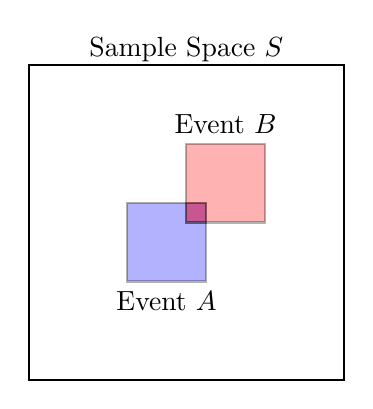
\begin{tikzpicture}

% Draw the sample space S as a large square
\draw[thick] (0,0) rectangle (4,4);
\node at (2, 4.2) {Sample Space \( S \)};

% Draw event A as a smaller square inside S
\draw[thick, fill=blue, opacity=0.3] (1.25, 1.25) rectangle (2.25, 2.25);
\node at (1.75, 1.0) {Event \( A \)};

% Draw event B as another smaller square inside S
\draw[thick, fill=red, opacity=0.3] (2, 2) rectangle (3, 3);
\node at (2.5, 3.25) {Event \( B \)};

% Show intersection area A ∩ B
\draw[thick, fill=purple, opacity=0.3] (2, 2) rectangle (2.25, 2.25);
%\node at (2, 2) {\small $A \cap B$};

\end{tikzpicture}
\end{minipage} %
\hfill 
\begin{minipage}{.45\textwidth}

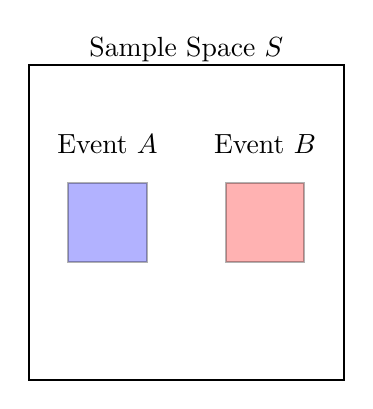
\begin{tikzpicture}

% Draw the sample space S as a large square
\draw[thick] (0,0) rectangle (4,4);
\node at (2, 4.2) {Sample Space \( S \)};

% Draw event A as a smaller square inside S
\draw[thick, fill=blue, opacity=0.3] (0.5, 1.5) rectangle (1.5, 2.5);
\node at (1, 3) {Event \( A \)};

% Draw event B 
\draw[thick, fill=red, opacity=0.3] (2.5, 1.5) rectangle (3.5, 2.5);
\node at (3, 3) {Event \( B \)};

%% Show intersection area A ∩ B
%\draw[thick, fill=purple, opacity=0.3] (1.5, 1.5) rectangle (2.5, 2.5);
%\node at (2, 2) {$A \cap B$};

\end{tikzpicture}
\end{minipage} %

\vfill 
\pause 

\begin{minipage}{.45\textwidth}
\begin{center}
These events are \textbf{independent}.

\begin{align*}
P(A \cap B) &= P(A) \; P(B) \\
&= \frac{1}{16} \cdot \frac{1}{16}   = \frac{1}{256} 
\end{align*}
\end{center}
\end{minipage} %
\hfill 
\begin{minipage}{.45\textwidth}

These events are \textbf{dependent}.

\begin{align*}
P(A \cap B) &= 0  \\
& \neq  P(A) \; P(B) = \frac{1}{16} \cdot \frac{1}{16}
\end{align*}
\end{minipage} %
\vfill 
\pause 
\colorbox{orange!30}{\textbf{Remark.}} Dependence doesn't need to be so extreme. The left  figure would depict dependence even if we just pulled the blue and red squares apart from each other ever so slightly.  Likewise if we pushed them closer together slightly.
\end{frame}

\begin{frame}{Note on overall grades}

The averages posted on Brightspace are cumulative.
\vfill 
\begin{figure}
\includegraphics[width=\textwidth]{images/overall_grades}	
\end{figure}

\vfill 
	
\end{frame}


\begin{frame}[standout]
Today's quiz
\end{frame}

\begin{frame}
\small 

\begin{myredbox}[title=\text{Reading Quiz (Random Variables)}]


\begin{enumerate}
	\item Let $(S,P)$ be a probability space. What is the name for a function defined on $S$?
	\item Let $(S,P)$ be the probability space formed by rolling a pair of die.   Let $X$ be a random variable defined on this space as the sum of the values of the two dice. 
	\begin{enumerate}
	\item[a.] (True/false)  $P(X=8) = P(\set{s \in S : X(s) = 8})$.
	\item[b.] (True/false)  $P(X=8) = P(\set{(2,6), (3,5), (4,4), (5,3), (6,2)})$.
	\item[c.] (True/false)  $P(X=8) = \frac{5}{36}$.
	\item[d.] (True/false)
		$P(X \geq 8) = P(\set{s \in S : X(s) \geq 8})$.
	\end{enumerate}
\end{enumerate}
\end{myredbox}

\vspace{-.2cm}

\begin{mygreenbox}[title=\text{Problems Quiz (Binomial Coefficients, Incl/Excl, Intro to Probability)}]

\begin{enumerate}
\item Determine the number of 2 element subsets of $\set{a,b,c,d,e}$ in two different ways. 
\item What is the probability of getting a full house in a 5-card poker hand?  A full house is three cards with one common rank and two other cards of another common rank, such as three queens and two 4s.  (Note: you do not need to justify your answer or simplify binomial coefficients.)
\end{enumerate}

\end{mygreenbox}
	
\end{frame}


%\begin{frame}[standout]
%Introduction to Probability: \\
%Review Of Samples and Events
%\end{frame}

%\begin{frame}[standout]
%TODO: Point out slide 
%\end{frame}


\begin{frame}[standout]
Thoughts on random variables
\end{frame}



\begin{frame}{Random Variables}
\small 

\colorbox{green!30}{\textbf{Key concept.}} A \textbf{random variable} is a function on the sample space of a probability space.

\vfill 


\colorbox{yellow!30}{\textbf{Example.}} Suppose we flip four coins.  The sample space consists of 16 outcomes (see below).  We could define a random variable (function) that takes the value \green{green} whenever exactly two of the coins are heads, and \red{red} otherwise.

\begin{center}
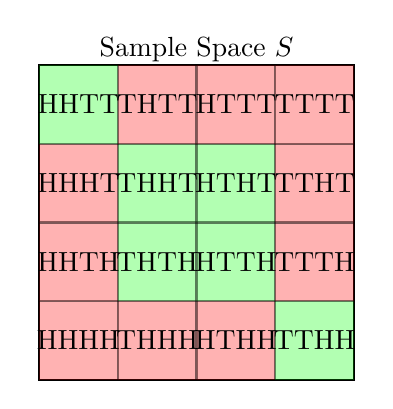
\begin{tikzpicture}

% Draw the sample space S as a large square
\draw[thick] (0,0) rectangle (4,4);
\node at (2, 4.2) {Sample Space \( S \)};

% Row 4
\draw[thick, fill=red, opacity=0.3] (0, 0) rectangle (1,1);
\node at (0.5, 0.5) {HHHH};

\draw[thick, fill=red, opacity=0.3] (1, 0) rectangle (2,1);
\node at (1.5, 0.5) {THHH};

\draw[thick, fill=red, opacity=0.3] (2, 0) rectangle (3,1);
\node at (2.5, 0.5) {HTHH};

\draw[thick, fill=green, opacity=0.3] (3, 0) rectangle (4,1);
\node at (3.5, 0.5) {TTHH};


% Row 3
\draw[thick, fill=red, opacity=0.3] (0, 1) rectangle (1,2);
\node at (0.5, 1.5) {HHTH};

\draw[thick, fill=green, opacity=0.3] (1, 1) rectangle (2,2);
\node at (1.5, 1.5) {THTH};

\draw[thick, fill=green, opacity=0.3] (2, 1) rectangle (3,2);
\node at (2.5, 1.5) {HTTH};

\draw[thick, fill=red, opacity=0.3] (3, 1) rectangle (4,2);
\node at (3.5, 1.5) {TTTH};


% Row 2
\draw[thick, fill=red, opacity=0.3] (0, 2) rectangle (1,3);
\node at (0.5, 2.5) {HHHT};

\draw[thick, fill=green, opacity=0.3] (1, 2) rectangle (2,3);
\node at (1.5, 2.5) {THHT};

\draw[thick, fill=green, opacity=0.3] (2, 2) rectangle (3,3);
\node at (2.5, 2.5) {HTHT};

\draw[thick, fill=red, opacity=0.3] (3, 2) rectangle (4,3);
\node at (3.5, 2.5) {TTHT};


% Row 1
\draw[thick, fill=green, opacity=0.3] (0, 3) rectangle (1,4);
\node at (0.5, 3.5) {HHTT};

\draw[thick, fill=red, opacity=0.3] (1, 3) rectangle (2,4);
\node at (1.5, 3.5) {THTT};

\draw[thick, fill=red, opacity=0.3] (2, 3) rectangle (3,4);
\node at (2.5, 3.5) {HTTT};

\draw[thick, fill=red, opacity=0.3] (3, 3) rectangle (4,4);
\node at (3.5, 3.5) {TTTT};
\end{tikzpicture}
\end{center}


\end{frame}

\begin{frame}{Binomial Random Variables}

\begin{myredbox}[title=\text{Problem (Quality Control in Manufacturing)}]

\begin{minipage}{.8\textwidth}
A factory produces \textbf{LED bulbs}, and 1\% of them are defective. A random sample of 20 bulbs is shipped to a customer.
\begin{enumerate}
	\item  What is the probability that \textbf{exactly 0} of the 20 bulbs are defective?  
	\item What is the probability that \textbf{no more than 1} bulb is defective? 
\end{enumerate}
  
\end{minipage} % 
\hfill 
\begin{minipage}{.18\textwidth}
\includegraphics[width=\textwidth]{images/broken_bulb}  
\end{minipage} % 
 


\end{myredbox}

\vfill \vfill 

\begin{mygreenbox}[title=\text{Tool: Binomial Random Variables}]

A binomial random variable $X$ gives the number of successes in a sequence of $n$ independent experiments, each asking a yes–no question, where success occurs with probability $p$.  

\[ P(X=x) = \binom{n}{x} p^x (1-p)^{n-x} \]
\end{mygreenbox}
\end{frame}


\begin{frame}


\vfill 
\begin{myyellowbox}[title=Solution]
Let:  
\begin{itemize}
\item $ n = 20$ $\rightarrow$ total bulbs tested. 
\item $ p = 0.01$ $\rightarrow$ probability of a bulb being defective.
\item   $X$ 	$\rightarrow$ the number of defective bulbs, which follows a \textbf{binomial distribution}
\end{itemize}

\begin{enumerate}
	\item The probability that \textbf{exactly 0} of the 20 bulbs are defective is
	\[P(X = 0) = \binom{20}{0} (0.01)^0 (0.99)^{20} = 0.8179\]
	\item The probability that \textbf{no more than 1} bulb is defective is
	\begin{align*}
	P(X \leq 1) & = P(X = 0) + P(X = 1) \\
	&= \binom{20}{0} (0.01)^0 (0.99)^{20} + \binom{20}{1} (0.01)^1 (0.99)^{19} \\
	& = 0.8179 + 0.1652 = 0.9831
	\end{align*}

\end{enumerate}
\end{myyellowbox}
	
\end{frame}




\begin{frame}[standout]
Group exercises
\end{frame}

\begin{frame}
\footnotesize 
\vfill 
\begin{columns}
\begin{column}{0.33\textwidth}
aaron.loomis: 8 \\ 
adam.wyszynski: 13 \\ 
alexander.goetz: 15 \\ 
alexander.knutson: 17 \\ 
anthony.mann: 4 \\ 
blake.leone: 21 \\ 
bridger.voss: 6 \\ 
caitlin.hermanson: 2 \\ 
cameron.wittrock: 10 \\ 
carsten.brooks: 19 \\ 
carver.wambold: 3 \\ 
colter.huber: 18 \\ 
conner.reed1: 13 \\ 
connor.mizner: 6 \\ 
connor.yetter: 11 \\ 
derek.price4: 21 \\ 
devon.maurer: 9 \\ 
emmeri.grooms: 15 \\ 
erik.moore3: 9 \\ 
ethan.johnson18: 12 \\ 
evan.barth: 4 \\\end{column}
\begin{column}{0.33\textwidth}
evan.schoening: 20 \\ 
griffin.short: 16 \\ 
jack.fry: 7 \\ 
jacob.ketola: 5 \\ 
jacob.ruiz1: 19 \\ 
jacob.shepherd1: 17 \\ 
jada.zorn: 1 \\ 
jakob.kominsky: 12 \\ 
james.brubaker: 9 \\ 
jeremiah.mackey: 14 \\ 
jett.girard: 15 \\ 
john.fotheringham: 14 \\ 
jonas.zeiler: 20 \\ 
joseph.mergenthaler: 3 \\ 
joseph.triem: 2 \\ 
julia.larsen: 3 \\ 
justice.mosso: 1 \\ 
kaden.price: 2 \\ 
lucas.jones6: 8 \\ 
luka.derry: 5 \\ 
luke.donaldson1: 1 \\\end{column}
\begin{column}{0.33\textwidth}
lynsey.read: 7 \\ 
mason.barnocky: 10 \\ 
matthew.nagel: 19 \\ 
micaylyn.parker: 7 \\ 
michael.oswald: 11 \\ 
nolan.scott1: 10 \\ 
owen.obrien: 11 \\ 
pendleton.johnston: 18 \\ 
peter.buckley1: 16 \\ 
reid.pickert: 13 \\ 
ryan.barrett2: 16 \\ 
samuel.hemmen: 21 \\ 
samuel.mosier: 5 \\ 
samuel.rollins: 18 \\ 
sarah.periolat: 6 \\ 
timothy.true: 12 \\ 
tristan.nogacki: 4 \\ 
tyler.broesel: 17 \\ 
william.elder1: 14 \\ 
yebin.wallace: 8 \\ 
zeke.baumann: 20 \\\end{column}
\end{columns}
\vfill
\end{frame}


\begin{frame}{Group exercises}

\begin{enumerate}
	\item \small  A fair coin is flipped three times. This is modeled by a probability space $(S,P)$ where $S$ contains the eight lists from $(H,H,H)$ to $(T,T,T)$, all with probability $\frac{1}{8}$.  Let $X$ denote the number of times we see TAILS.
	\begin{itemize} \footnotesize 
	\item[a.] Write $X$ explicitly as a function defined on $S$.
	\item[b.] Write the event \enquote{X is odd} as a set.
	\item[c.] Calculate $P(\text{X is odd})$.
	%\item[d.] Let $Y$ denote the number of times we see HEADS.  Are $X$ and $Y$ independent?  Provide the intuition, and then a mathematical argument.
	\end{itemize}
	\item \small  
	A basketball player has a 75\% chance of making a free throw. During a game, the player takes 10 free throws. Model the number of free throws made as a binomial random variable. 
		\begin{itemize}\footnotesize  
		\item[a.] What is the probability that the player makes exactly 8 free throws?
		\item[b.] What is the probability that the player makes at least 7 free throws?
		\end{itemize}
	\item  \small  For each situation below, determine whether $X$ and $Y$ independent. First provide the intuition, and then provide a mathematical argument. 
	\begin{itemize} \footnotesize
	\item[a.] A fair coin is flipped three times. Let $X$ be the number of heads and $Y$ be the number of tails. 
	\item[b.] A card is drawn at random from a standard deck of 52 cards. Let $X$ be the rank of the card (from 2 to ace) and $Y$ be the suit of the card.
	\item[c.] Two cards are drawn at random (without replacement) from a standard deck of 52 cards. Let $X$ be the rank of the first card and $Y$ be the rank of the second card.
	\end{itemize} 
\end{enumerate}

\end{frame}




\end{document}
